\chapter{Literature Review}\label{ch:LitReview}

\section{Introduction}

If one thinks of \glsfull{IB} and literature, a number of large firms and their business strategies spring to mind.
What choices did they make and what will they do in the future? 
Many companies respond to current events in the choices they make.
Even very large~\gls{MNE}, who have the resources to engage in scenario planning or other costly and time consuming methods to prepare for the eventual future, can be caught off guard.
This is illustrated by Microsoft having to announce~\citep{FT:2013} a broad reorganisation of the company to combat the decline in PC sales.  %(in 2013)
These are economic challenges, brought upon the company due to changes in consumer preference or consumer behaviour.
But what happens if the rules change? \\
The introduction of \gls{trips} should have had an effect on the way business was done with regard to \glsfull{IP} rights.
The change in rules was forced on the businesses. 
This change was imposed on the \glsfull{IB} by institutions such as the~\wto. 
It were the institutions that created the new rules and companies had to live with these new rules.
Many more global impacting trade rules are set by the~\wto. 
In this section the~\wto~will be conceptualised as an institution with the aide of institutional theory.
The concept of institutional theory and institutions will be researched.
Also the predominant IB strategy literature will be visited to provide a basis for the reactions firms have to such changes that institutions as the~\wto~present to MNEs. 



%Does the \wto~ effect firms from different backgrounds differently? 

\section{Institutions, Organisations and Institutional Theory}\label{sec:InTh}

\newcommand{\inth}{institutional theory}
To grasp the concept of \inth~first institutions and organisations have to be clearly understood. These two are the basis for the concept of \inth.

\subsection{Institutions}

The term `institution' is defined in the dictionary as `an organisation founded for  religious, educational, professional, or social purpose' or `an established law or practice'\footnote{Oxford Dictionary of English 3rd edition}.
It is the concept of an `established law or practice' that is of interest here.\\
IB literature is replete with definitions of what an institution construes.
Among sociologists such as Scott the definition of institutions is still a work in progress.
Starting in 1995 Scott defines institutions as: 
\begin{quote}Institutions consist of cognitive normative and regulative structures and activities that provide stability and meaning to social behaviour. Institutions are transported by various carriers --cultures, structures and routines-- and they operate at multiple levels 
~\citep{Scott:1995}
\end{quote}
Then starting in 2008 Scott has a slightly different definition:
\begin{quote}
Institutions are social structures that have attained a high degree of resilience [and are] composed of cultural-cognitive, normative, and regulative elements that, together with associated activities and resources, provide stability and meaning to social life~\citep{Scott:2010us,Scott:2008}
\end{quote}

Fligstein, like Scott also with a sociology background, articulates:
 \begin{quote} ``rules and shared meanings \ldots that define social relationships, help define who occupies what position in those relationships and guide interaction by giving actors cognitive frames or sets of meanings to interpret the behaviour of others''~\citep{Fligstein:2001dj}.
\end{quote}

North, being an economist, provides a somewhat different view on the concept of institutions as:
\begin{quote} The rules of the game in our society or more formal the humanly devised constraints that shape human interaction. In consequence they structure incentives in human exchange, wether political, social or economic~\citep{North:1990vl}
\end{quote}

\cite{North:1990vl} summarised institutions as the `rules of the game'. 
This apt summary is often used as an explanation for institutions in literature~\citep{Peng:2008b,Westney:2005vv,Jackson:2008cz,Newman:2000fc,vanEssen:2012cw,Hotho:2012uu}.
The latter of the definitions (by North) have a more economically orientated standpoint. The aforementioned definitions by~\citep{Fligstein:2001dj,Scott:2008} are, of a more sociologist point of view.
A host of others have also defined institutions. 
An overview of those definitions can be found in~\citep{Scott:2010us}. 
Their definition depends on their background and their varying attention to one or the another side of the institutional element~\citep{Scott:2010us}.\\
Some scholars identified that \inth~could become an interdisciplinary turf battle~\citep{Peng:2009vt} as \inth~has both sociological and economical aspects and hence the exact definition of the concept of the institution.
\cite{Peng:2009vt} also adds to the institutional discussion by stating:
``More broadly speaking, institutions serve to reduce uncertainty for different actors by conditioning the ruling norms of firm behaviours and defining the boundaries of what is considered legitimate''~\citep[p.66]{Peng:2008us}.
No preference is given in this thesis to either of the conceptualisations of institutions. 

%In line with~\cite{Peng:2009vt} this thesis will ``use an integrative approach, drawing on the best insights from both economics and sociology as well as other allied disciplines''.

One commonality in the discussion surrounding institutions, is the identification of three different types of institutions. 
\cite{Scott:2005us} uses the terms `pillars' or `elements' to typify the different types of institutions.
The same three types of institutions have been identified by others such as~\cite{Peng:2008us} with the term `dimensions'.

The following are the conceptualisations of Scott, his three pillars are:
\begin{description}\label{desc:pillars}
\item [regulative] Regulative elements stress rule-setting, monitoring, and sanctioning activities. 
 Regulative elements are more formalised, more explicit, more easily planned and strategically manipulated. 
 In this pillar laws, rules and regulations are set and enforced thorough force, fear or expedience~\citep{Scott:2005us,Scott:2010us,Scott:2008tk}.
\item [normative] Normative elements introduce a prescriptive, evaluative, and obligatory dimension into social life.
Actors are viewed as social persons who care deeply about their relations to others and adherence to the guidelines provided by their own identity. 
These normative systems include both values and norms and define goals and objectives. 
Decisions are responsive not only to `instrumental’ considerations but to the logic of `appropriateness’~\citep{Scott:2005us,Scott:2010us,Scott:2008tk}.
\item [cultural-cognitive] cultural-cognitive elements emphasise the “shared conceptions that constitute the nature of social reality and the frames though which meaning is made.
The elements are cultural because they are socially constructed symbolic representations.
they are cognitive in that they provide vital templates for framing individual perceptions and decisions~\citep{Scott:2005us,Scott:2010us,Scott:2008tk}.
\end{description}

Concluding, institutions can have different forms, or pillars as Scott named them. 
The way in which one complies to these institutions and the mechanisms employed to comply with institutions is explained in the section~\ref{sec:InstTheory}.

\subsection{Organisations} 

As seen, institutions can influence organisations. 
But what are these organisations?
The dictionary defines organisations as: `an organised group of people with a particular purpose, such as a business or government department'\footnote{Oxford Dictionary of English 3rd edition}. 
\citep[p.14]{Scott:2005us} defines an organisation as: ``organisations were recognised to be `rationalised' systems—sets of roles and associated activities laid out to reflect means-ends relationships oriented to the pursuit of specified goals''.\\
Among scholars of \inth~there has been a debate on the use of the term `organisations'. 
Some prefer the term `organisational field'~\citep{DiMaggio:1983wt,Westney:2005vv}.
Here the purpose is, to have a clear understanding, that organisations can be the international firms (or \glspl{MNE}).
Firms are subject to the institutions that are governing their business fields (fields of play).
The, so called, organisational fields are the set of organisations or companies that do business as suppliers and (product) consumers.



\subsection{Institutional Theory}\label{sec:InstTheory}


Institutional theory begins with the premise that organisations are a social, as well as a technical phenomena~\citep{Westney:2005vv}.
This means that the pressures from institutions (rules, regulations, norms etc.) are not interpreted on their technical merit alone.
The shape and form of the pressures from institutions can differ.
\cite{Scott:2008tk} identifies this by saying that, the basis of order, the motives for compliance, the logics of action, the mechanisms and the indicators employed, differ among the institutional pillars. 
Organisations comply to the pressures of institutions (rules, norms and meanings)~\citep{Scott:2008tk}.
Institutional theory takes thus into account, the context of both the organisation and the institutional environment.
However one has to keep in mind that organisations cannot be seen as rational~\citep{Westney:2005vv}.
To counter these observations, \inth~does not look inside the organisation, it looks at the social context and focusses on ``\iso within the institutional environment''~\citep{Zucker:1987vn,Westney:2005vv}.\\
Institutional theory can thus contribute in, connecting the context of a firm to the type of responses firms use to act on pressure from institutions.
The form in which organisations respond to these institutions changes is often similar.
\cite{DiMaggio:1983wt} dubbed these similarities \iso and introduced the concept of isomorphic pressures for this process.
Isomorphic pressures refer to influences of conformity exerted on firms by the government, professional associations and other external constituents that define or prescribe socially acceptable economic behaviour~\citep{Scott:2001tt}.
The reason for this behaviour, institutional theorists argue, lies in the fact that organisations in the same population or industry tend toward similarity (\isos) over time, because they conform to many common influences and are interpenetrated by relationships that diffuse common knowledge and understandings~\citep{DiMaggio:1983wt,Meyer:1978if,Jepperson:1991tu,Oliver:1988un,Scott:1987uq}.
It is the environment populated by organisations that has relationships, not simply transactions, that is the basis of organisations towards alternative ways of organising themselves, thereby influencing organisations towards \iso\footnote{\iso can be defined as `the adoption of structures and processes prevailing in other organisations within the relevant environment'~\citep{Zucker:1987vn}}~\citep{Westney:2005vv,DiMaggio:1983wt,Zucker:1987vn}. 
Therefor institutional theory focuses on the reproduction or imitation of organisational structures, activities, and routines in response to state pressures, the expectations of professions, or collective norms of the institutional environment~\citep{DiMaggio:1983wt,Zucker:1987vn}.
The mechanisms that support this process of institutionalisation, the social forces that energise the diffusion~\citep{DiMaggio:1983wt}, can be summarised in three~\isos.
The three \isos, the mechanisms through which organisations comply with the rules, norms and meanings, imposed by institutions are:


\begin{description}
\item[Coercive \iso] organisational patterns are imposed on on organisations by a more powerful authority 
\item[normative \iso] appropriate organisational patterns are championed by professional groups and organisations
\item[mimetic \iso] where organisations respond to uncertainty by adopting the patterns of other organisations that are deemed `successful' in that kind of environment~\citep{Westney:2005vv,DiMaggio:1983wt,Peng:2008us,Kostova:1999wt,Scott:2001tt}
\end{description}
The basis of choice for firms for either alternative \isos can be found in the basis of compliance (with the institutional change)~\citep{Scott:2005us}.
The three compliance possibilities that has Scott identified are:
\begin{enumerate}
  \item expedience
  \item social obligation
  \item on a taken for granted basis
\end{enumerate}
The relationship between the \isos their compliance basis is summarised in Table~\ref{tab:Pillars}. 
It also gives an overview of the pillars and their attributes with regard to compliance basis, mechanisms of~\iso.
\cite{Scott:2005us} talks here about pillars of institutions.
Further information on how organisations internally deal with institutional pressure can be found in Section~\ref{sec:firmResponses}.
%This has been summarised in Table~\ref{tab:Pillars}.
These three compliance basis correspond nicely to the pillars of institutions~\ref{desc:pillars}.



\begin{table}[htp]
\setlength{\tabcolsep}{4pt}  % slight reduction from default value
\caption[Pillar of Institutions]{Pillar of Institutions (source:adapted from~\citep{Scott:1995})}\label{tab:Pillars}
\smallskip
\begin{tabularx}{\textwidth}{@{} l
  >{\hsize=0.92\hsize}Y      % One can vary widths of "X" column types, 
  >{\hsize=1.04\hsize}Y      % as long as the factors  add up to number of 
  >{\hsize=1.04\hsize}Y @{}} % columns of type "X" 
\toprule
 & Regulative & Normative& Cultural-cognitive \\ 
\midrule
Basis of compliance  &Expedience& Social obligation & Take-for-grantedness \linebreak Shared understanding\\
Basis of order & Regulative rules& Binding Expectations &Constitutive Schema\\
Mechanisms & Coercive     &Normative & Mimetic\\
Logic &instrumentally     & Appropriateness& Orthodoxy\\
Indicators & Rules \linebreak Laws  \linebreak Sanctions    &Certifications \linebreak Accreditation  & Common beliefs\linebreak Shared logic of action\\
Basis of legitimacy      &Legally sanctioned & Morally governed & Comprehensible \linebreak Recognisable \linebreak Culturally supported\\
Supported by &Economists  & Early Sociologists & Late Sociologists\\
Primary Propagandists     & North & Selznick & DiMaggio and Powell, Scott\\
Degree of formality       &Formal institutions &Informal institutions&Informal institutions\\
\bottomrule
\end{tabularx}
\end{table}

The basis of compliance and the mechanisms (or~\iso) with which organisations employ themselves are relative to the same pillars (see table~\ref{tab:Pillars}).
\cite{North:1990vl} also identified different institutions. 
However his distinction was along the line of formal and informal institutions.
The theories of North and Scott are somewhat complementary~\citep{Peng:2009vt}. 
For that fact, the concepts of North and Scott are presented in the same table (\ref{tab:Pillars}).
Where North's `formal' institutions refer to Scott's laws, rules and regulations (regulative pillar), the informal are somewhat consistent with the normative and social-cognitive pillars of~\cite{Scott:1995}.

The application of institutional theory is `on the rise'~\citep{Westney:2011ih}.
Not solely because it can be a highly insightful approach when probing into organisational strategies in Asia~\citep{Hoskisson:2000wd}, but also because is gives a handle why the same rules (regulations) have different outcomes when imposed on different societies~\citep{North:1990vl}.
International firms can have these issues because they have different `rules of the game' in different societies (countries or regions), but also because they operate in different countries and under different (formal) rules and regulations. 
The rise of institutional theory provided a way of interpreting these developments with an alternative to the model of the firm and its environment that has long dominated strategy research~\citep{Westney:2011ih}.
Applying this theory to \glsfull{EE} and \glsfull{AE} the following working propositions can be derived.

\begin{subtheorem}{WP} 
\begin{WP}\label{wp:same_same}
Firms in the same economic region and in similar industries (Services or Manufacturing) are likely to have a homogenise response to changes in the institutional environment%
\end{WP}
\begin{WP}\label{wp:same_Eco_Diff_Ind}
Firms in the same economic region, but in different industries (Services or Manufacturing) are likely to have a heterogenous response to changes in the institutional environment%
\end{WP}
\begin{WP}\label{wp:same_Ind_Diff_Eco}
Firms in the same industry (Services or Manufacturing) but in different economic regions are expected to have a heterogenous response to changes in the institutional environment%
\end{WP}
\end{subtheorem}

\subsection{Multiple embeddedness}

Globalisation impinges on MNEs and their complex interdependencies within and between multiple host locations as well as on their internal hierarchies~\citep{Meyer:2011vt}.
The intricate dependancies on the level of institutions, resources and home and host country are shown in figure~\ref{fig:Meyer}
As such the MNEs are likely to be subject to a selection of different and possibly contradictory influences, that originate from the different environments they operate in~\citep{Westney:2005vv}.
Firms respond to these \iso pulls by setting up formal structures to cope with or replicate the environmental pressures~\citep{Westney:2005vv}. 
On the other hand, these differences over countries within one organisation can cause problems.
\mne must balance ‘internal’ embeddedness within the MNE network, with their ‘external’ embeddedness in the host milieu~\citep{Meyer:2011vt}.
These can be in the form of corporate legal departments \iso to law firms in the local domain or public relation offices staffed with former public officials~\citep{Westney:2005vv}. 
The opportunity for clashes is not limited to \mne and external pressures.
Within the \mne there is the potential of clashes. 
Managers in the home country can be rooted in a different institutional context that can lead them to pursue different strategies for the firm, rather than adapt to these local settings~\citep{Jackson:2008cz}.
The resource constraints that firms face could be managerial.
This might possible limit the growth of a company.
The phenomenon is has been by described by~\citep{Hutzschenreuter:2011bv} and is referred to as the ‘Penrose effect’. 
Limited resources mean that firms often experience a trade-off between product diversification and international diversification~\citep{Dunning:2008}.
The resulting clashes can create an endemic potential for strategic conflict~\citep{Jackson:2008cz}.

\begin{figure}[htbp] 
	\centering
	\includegraphics[width=0.8\textwidth]{meyer.png}
 	\caption[Multinational enterprises and local context]{Multinational enterprises and local context (source:~\cite{Meyer:2011vt})}\label{fig:Meyer}
\end{figure}

Multiple embeddedness on the other hand, can assist the \mne.
International firms could organise themselves to take full advantage of the differences in local rules and regulations.
Firms need to manage not just their corporate networks, but also their external networks~\citep{Meyer:2011vt}. 
MNEs may therefore focus certain activities in their home country in order to utilise certain institutional resources~\citep{Jackson:2008cz}.\\
Or as~\citep{Meyer:2011vt} states: given that many larger MNEs are a complex aggregation of a large number of constituent subsidiaries, such multiple embeddedness generates trade-offs between external and internal embeddedness, since each subsidiary must reconcile the interests of its parent with those of its local business interests.
Here the tax-breaks (in 2013) that Apple profited from in Ireland and the US springs to mind.
This ability to create, transfer, recombine, and exploit resources across international borders is one of the key reasons for existence of the \mne, their value creation is based on international arbitrage~\citep{Meyer:2011vt}.
The embeddedness that firms have to respond to may become a barrier to enterprise survival~\citep{Newman:2000fc}, on the other hand \me can provide\glspl{MNE} inherently with opportunities as well.
Due to the multiple embeddedness of many MNE's the homogeneity in firm responses is likely over different (economic) regions. 
This observation leads to the following working proposition.


\begin{WP}
Multiple embeddedness is expected to have a homogenising effect on the responses of firms in similar industries across different economic regions. 
\end{WP}


%---------------- Aantekeningen---------------------------------------------------------%%%%%%


%The central argument with regard to institutions is that “organisations conform to the rules and beliefs systems in the environment because this isomorphism (regulatory, cognitive and normative) earns them legitimacy.
%Not only have more scholars have come to realise that institutions matter and, that strategy research cannot just focus on industry conditions and firm resources alone~\cite{Powell:1991wn,Scott:2001tt}.
%The point is organisations consist of relations not of transactions~\cite{Westney:2005vv}. 
%This changes the dynamic of organisations.
%Institutions are pervasive in that they are capable of shaping the behaviours of multiple organisations (i.e. individuals, firms, industries, and~\glspl{NGO})~\cite{Peng:2008tb}.  
%\cite{North:1990vl} defines the same phenomena as:
%Institutional factors function as the formal and informal ``rules of the game'' that socially constrain contracting practices between the \gls{BoD} and executives.
%The formal and informal institutions can be summarised as in table~\ref{tab:Pillars}
%Firms do not only have to look at their resources and capabilities~\cite{Barney:1991ur}, but have to look at ``the rules of the game''~\cite{Scott:2001tt}. 
%These so called rules include the environment that the firm \mne~has to adhere to.
%Institutions are the formal and informal rules of the game~\cite{North:1990vl}. These institutions are influencing the decision making process in~\gls{IB}.
%Diffusion (zie Lawrence 2006)
%A range of institutional writings have located diffusion as a central dynamic in the institutionalization of a structure or practice (Greenwood et al., 2002; Tolbert \& Zucker, 1996; Zucker, 1987)
%When markets work smoothly in developed economies, ``the market-supporting institutions are almost invisible``.~\cite{McMillan:2008}
%The effect of institutions on strategy can be seen most obviously in the asian economies~\cite{Peng:2002}.
%Where \rbv~looked solely at the firm in a set environment \ibv~also takes the surroundings into account. These surroundings are the institutions that govern the environment the \mne~is playing the game. \\
%According to~\cite{Peng:2003} unfortunately, little is known about how organisations make strategic choices when confronting such large-scale institutional transitions.

\section{World Trade Organisation}

%Whether the \wto~can be seen as an institution is investigated based on various literature. 

To be able to define the \wto~one has to look at what the \glsfull{WTO} actually is.
A brief history of the \wto~will be presented in this chapter, as well as the various roles the \wto~has and the different life cycles that exist with in the rules setting environment within the \wto.

The \gls{WTO}~was only established on January 1st 1995 under the Uruguay multilateral trade rounds.
After World War II much needed to change. 
The world had to come together. 
Hence global organisations were created tasked with rebuilding the world and ensuring its enduring peace. 
For this grand purpose the~\gls{un} was founded in 1944 but also the~\gls{IMF} and World Bank.\\
Around the same time an organisation, under the wings of the \gls{un}, tasked with trade was to be established named. 
This organisation has the name~\gls{ito}. 
However the~\gls{ito} never saw the light of day, for the treaty governing this \gls{ito}, was not approved by the United States and a few other countries. 
Instead, a provisional agreement on tariffs and trade rules, the \gls{gatt} was reached. 
This agreement went into effect in 1948.
Before the establishment of the~\wto, the \gls{gatt} was the primary body delegated with international trade. 
\textcolor{red}{The ``provisional''~\gls{gatt} treaty became the principal set of rules governing international trade until the \gls{WTO}.}%\\
The \gls{WTO} incorporated many `Uruguay Round' changes such as newly formed negotiated reforms, bodies to oversee the new trade agreements, a stronger dispute resolution procedure, a regular review of members’ trade policies and many other committees and councils. 
In contrast to the \gls{gatt}, the \gls{WTO} was created as a permanent structure, with `members' instead of `contracting parties'~\cite{Fergusson:2007ws}.\\
Nowadays, at its heart are the WTO agreements, negotiated and signed by the bulk of the world’s trading nations. 
The \wto~sets rules or legal agreements for international commerce and finally it helps to settle disputes~\cite{WTO:2012}.



\subsection[WTO Life cycles]{\wto~life cycles}
The WTO agreements are reached through a three step process. 
Understanding this process (the life cycles) is very relevant for, only at the formulation phase of the process, actual influence on the content of the rules of the agreement can be had~\citep{WTO:2012}.
Within these life cycles the various roles, the~\wto~has, will become relevant.
The three phases of the decision-making lifecycle, within the \wto, consist of~\citep{Lawton:2009vw}:

\begin{itemize}
\item formulation of trade rules
\item implementation of those rules
\item enforcement of the rules
\end{itemize}

Figure~\ref{fig:Lawton} gives an indication the relationships between the three phases. 
The phase where new members enter into the \wto~as is not mentioned, as this is considered not within scope.

\begin{figure}
\centering
\tikzsetnextfilename{WTO_Live_Cycles}
\begin{tikzpicture}[scale=0.8, transform shape]
% STYLES
\tikzset{%
    force/.style={%
    node distance = 1cm, 
    %auto,
    rectangle,
    rounded corners, 
    fill=black!10,
    node distance=3cm,
    inner sep=5pt, 
    text width=4cm, 
    text badly centered, 
    minimum height=1.3cm}
    }
\tikzset{%
    dummy/.style={%
    node distance = 1cm, 
    %auto,
    %rectangle,
    %rounded corners, 
    %fill=black!10,
    %node distance=3cm,
    %inner sep=5pt, 
    %text width=4cm, 
    %text badly centered, 
    %minimum height=1.3cm
    }
             }
% Draw forces
\node [force] (NewMember) {New Member Accession};
\node [force, right=1cm of NewMember] (Rules) {Rule Formulation (Trade Rounds)};
\node [dummy, below=2cm of Rules] (dummy) {};
\node [force, left=1cm of dummy] (Enforcement) {Rule Enforcement};
\node [force, right=1cm of dummy] (Implement) {Rule Implementation};


% Draw the links between forces
\path[->,thick] 
(NewMember) edge (Rules)
(Rules) edge [bend left] (Implement)
(Implement) edge [bend left] (Enforcement)
(Enforcement) edge [bend left]  (Rules);

\end{tikzpicture} 

\caption[WTO life cycles]{\wto~lifecycles source:~\cite{Lawton:2009vw}}%
\label{fig:Lawton} %
\end{figure}


\subsubsection{Formulation Phase}\label{sec:WTO:formulation_phase}
In the formulation phase, the \wto~plays the role of facilitator. 
At this moment in the cycle new agreements are being formulated through negotiations among members~\citep{WTO:2012}.
It is widely acknowledged that \gls{IB} and \gls{NGO} actors attempted to shape these agreements through engagement with their national governments~\citep{Lawton:2009vw}.
One example of the influence that firms imposed on the negotiations\footnote{These were the Uruguay Round (1986-1994) negotiations} through their own government were the agreements dictated in \gls{trips}~\citep{Lawton:2009vw}.\\
In the formulation phase, the second role of the WTO is that of a negotiating forum~\citep{WorldTradeOrganization:2008tz}.
The \wto~can act as a court where members can appear before, to try and sort out trade problems they face with each other.
This can lead to numerous negotiations between the members. 
Everything the WTO does, is the result of negotiations~\citep{WorldTradeOrganization:2008tz}.
The WTO is currently host to new negotiation rounds, under the “Doha Development Agenda” launched in 2001~\citep{WTO:2012}.



\subsubsection{Implementation Phase}
Once the member nations have come to an agreement on the sets of rules and regulations, these (\rr) have to be implemented. 
The implementations are a separate process in itself~\citep{WTO:2013}. 
The agreements need to be implemented and operationalised, this is a complex and nuanced process~\citep{Lawton:2009vw}.
During the implementation phase, the firms are experiencing the new rules and regulations for the first time. 
%If certain firms find the new \rr not as desired, these have to  to enter be amended.
Amendments to the rules and regulations can only be made once a regulation is challenged in the WTO disputes process~\citep{Lawton:2009vw}.
The \wto~members have considerable latitude in the exact way in which they implement the aforementioned rules. 
Tariffs and anti-dumping are chief among those rules where latitudes are applied~\citep{Hoda:2001, Reynolds:2009kc}.

The role of the WTO at this point in the process is that of a `set of rules'. 
This `set of rules' (negotiated agreements) are essentially contracts binding members to keep within the limits of these agreements on the topic of international trade.
The goal here is to facilitate and improve the flow of trade~\citep{WorldTradeOrganization:2008tz}.
The \wto~has also been active in settings rules for a number of intellectual properties such as copyrights, patents, trademarks and geographical names used to identify products~\citep{WTO:2013b}.


\subsubsection{Enforcement Phase}

The final phase of the life cycle within the WTO is the enforcement phase. 
Rules enforcement takes place at both the multilateral and national levels~\citep{Lawton:2009vw}. 
At the multilateral level, the WTO attempts to facilitate the diplomatic resolution of disputes between members over trade policies, but also provides a formal process for dispute settlements\footnote{This process is established by the Understanding on Rules and Procedures Governing the Settlement of Disputes also known as the \gls{DSU} (WTO, 2003, 55)~\citep{Lawton:2009vw}}.
It are the members, hence the nations, that have standing in the \wto.
So only nations are allowed to bring foreword the complaints of their individual firms to the \wto. 
Firms, at this point, play no part in the processes~\citep{WTO:2013c}.\\
On national level, the national government (within the \wto~boundaries) is responsible to ensure a `level' playing field for domestic industries, primarily through the use of antidumping, countervailing duty and safeguard investigations. 
National level enforcement is the responsibility of member governments’ domestic bureaucracy~\cite{Lawton:2009vw}.

The WTO has also the role of enforcer. 
This enforcer (or judicator) role is very important to give the agreements the power they need~\cite{Bown:2010}.
When necessary, albeit the negotiated agreements, members can bring disputes before the \wto~\citep{WTO:2013c}. 
Settling these disputes is the pillar of the \wto~trading system. The rules set by the \wto~are not as effective when there is no system to enforce these rules. The set of rules is not designed to pass judgement, the priority is to settle disputes (through consultations if possible)~\citep{WTO:2013a}.  
In 2008 only about 136 of the nearly 369 cases had reached the full panel process. Most of the rest have either been notified as settled ``out of court'' or remain in a prolonged consultation phase -- some since 1995~\citep{WTO:2012GATT}.\\
The life-cycles and thier actors have been summarised in table~\ref{tab:lawton:2009}.

\begin{table}[htb]
  \centering
  \caption[Multilateralism and the Multinational Enterprise]{Multilateralism and the Multinational Enterprise. Source~\cite{Lawton:2009vw}}\label{tab:lawton:2009}%
\begin{tabularx}{0.99\textwidth}{lXXX} 
 % \toprule
Actors &
Formulation Phase &
Implementation Phase &
Enforcement of Rules Phase \\
  \toprule 
%  \midrule
 WTO &
Facilitates negotiations &
Monitors compliance, provides information &
Operates disputes process, sanctions trade retaliation \\

Nation States &
Participates in negotiations &
Reforms domestic laws as necessary &
Acts as plaintiff or defendant in cases; acts as interested third party in other cases\\ 

Firms &
Non-market strategy to secure preferred policy outcomes of rules formulation &
Adjustment to the rules &
Adjustment to the rules \newline
Non-market strategy to gain redress for perceived unfairness by using the rules or amend the rules\\ 
  \bottomrule
\end{tabularx}
\end{table}









\subsection[Institutions and the WTO]{Institutions and the~\wto}\label{sec:institutions}  % conceptualisation of the WTO

The WTO, with its explicit accentuation of a ‘rules-based approach’, supported by norms of behaviour and in their implementation, can be and has been conceptualised 
by a number of authors through an institutional lens~\citep{Wilkinson:2013,Kim:2002wc,Herschinger:2012uk,Sokol:2009wr,Reich:2004tf,Bhagwati:2003,Irwin:2003}.
The rules and norms distinctions can be conceptualised using~\cite{North:1990vl} in formal and informal institutional categories (see also table~\ref{tab:Pillars}). 
In this paper, above all, the formal institutions are of interest. 
According to~\citep{North:1990vl} these formal institutions are laws, regulations and rules. 
These regulatory codes (laws, regulations and rules) are set by the governing institutions.
The codes though can be set at different levels.
Take the \gls{EU}, here the codes can be set on regional, national and even European level. \\
Belgium for example has a federal structure of government. 
Hence on codes are set on regional, thus federal level (in Flanders and Wallonia) and on national level. 
Both have their own governments and impose codes independently. 
Superseding the national level, Belgium has to adhere to the European laws, rules and regulations. 

On a global level, where trade is concerned, the~\wto~is the body that has the final say in the rules and regulations. 
The \wto~formulate and enforce the global trade rules and this should reduce uncertainty for organisations~\citep{Peng:2002ef}.
The uncertainty reduction is one of the key elements in the functioning of institutions and the primary raison d'être of many of them.
Clearly the \wto~tries to reduce the uncertainty for organisations by not only setting the rules but enforcing them as well.\\
Obviously the actions of institutions influence the decision making of organisations. 
This is also observed by~\cite{Peng:2002ef} and shown in figure~\ref{fig:Peng2000}. 
\cite{Peng:2000ut} discusses strategic choices in the form of the decision making.
%According to~\cite{Hotho:2012uu} institutions affect governance arrangements are most efficient, but they have little impact on how the game is played other than through the establishment of rules and regulations. 
The establishment of rules and regulations can be seen as the primary concern of institutions. 
Here we can observe that the rule setting role of the \wto~seamlessly fits within the confines of what~\cite{Hotho:2012uu} defines as institutions. 
Also according to~\citep{Hotho:2012uu,Jackson:2008cz} ``institutions, such as the \wto~are conceived of as factors that independently constrain or impact [\ldots] the cost of \gls{IB} activity''.\\
In the differentiation defined by~\cite{Scott:2001tt} the \wto~is seen as a Regulatory (or Coercive) (see table~\ref{tab:Pillars}) system or institution. 
Again the rules setting role of the \wto~give the \wto~the status of an institution according to~\cite{Scott:2001tt}.



\section{Firm responses}\label{sec:firmResponses}

\subsection{Responses to institutions}
As seen \inth in Section~\ref{sec:InstTheory} is a powerful tool.
In order to understand the influence of the \wto~on IB in the region of \gls{AE} and \gls{EE} in particular it is of importance to understand how firm react to `institutional change'.
According to~\cite{North:1990vl} institutional change may result from changes in the character and content of either or both of these, or their relevant enforcement mechanisms.

\subsubsection{First and second order changes}
Literature makes a distinction in first and second order changes when it comes to firm responses~\citep{Meyer:1995td}.
First order changes involve changes in processes, systems and or structures. These changes happen in periods of relative calm and tend to span extended periods of time~\citep{Dutton:1991gk,FoxWolfgramm:1998vu,Tushman:1985}.\\
Second order change however is associated with more radical, transformational and fundamental change.
It alters the business organisation at it's core~\citep{Meyer:1982ug,Meyer:1995td,Tushman:1985,Newman:2000fc}.
This leads to the next working proposition.

\begin{WP}\label{WP:WTO_rr_2nd-change}
The WTO~\rr are expected to incur only second order changes 
\end{WP}
Traditionally firms have to respond to changes in the business landscape due to market driven changes~\citep{Chittoor:2008cj}.\\
Now the change is initiated by institutions and this can lead to these aforementioned second order changes~\citep{Chittoor:2009jh}.
So in this case, it is not the market that forced the change, however is the market that, as a whole, has to adapt to the (same) change.
There is a relative paucity of research on how organisations transform themselves in the face of institutional transitions~\citep{Chittoor:2008cj}.\\

\subsubsection{Strategic Responses}
\cite{Cantwell:2009hg} provides a very intriguing insight in the different coping mechanism that firms employ in the face of institutional change.
According to~\cite{North:1990vl} institutional change may result from changes in the character and content of either or both of these, or their relevant enforcement mechanisms.
Among scholars notable contributions on the conception of how firm react to changes have been make by~\citep{Oliver:1991tm,Cantwell:2009hg}.
The broadest being~\cite{Oliver:1991tm} as seen in table~\ref{tab:Oliver:1991}, gives five basic reaction types.
The reactions are categorised from from passivity to increasing active resistance: acquiescence, compromise, avoidance, defiance, and manipulation~\citep{Oliver:1991tm}.

%%%%%%%%%%%%%%%%%%%%%%%%%%%%%%%%%%%
\begin{table}[htdp!]
  \caption[Strategic responses to institutional processes]{Strategic responses to institutional processes (source~\cite{Oliver:1991tm})}\label{tab:Oliver:1991}
\centering
\begin{tabular}{lll} 
  \toprule
	Strategies & Tactics & Examples \\ 
	\midrule
	          &Habit        &Following invisible, taken-for-granted norms\\
Acquiesce     &Imitate      &Mimicking institutional models\\
	          &Comply       &Obeying rules and accepting norms\\
	\\
	          &Balance       &Balancing the expectations of multiple constituents\\
Compromise    &Pacify        &Placating and accommodating institutional elements\\
	          &Bargain       &Negotiating with institutional stakeholders\\
	\\
	          &Conceal       &Disguising nonconformity\\
Avoid         &Buffer        &Loosening institutional attachments\\
              &Dismiss       &Ignoring explicit norms and values\\
    \\
              &Escape        &Changing goals, activities, or domains\\
Defy          &Challenge     &Contesting rules and requirements\\
              &Attack        &Assaulting the sources of institutional pressure\\
   \\  
              &Co-opt        &Importing influential constituents\\
Manipulate    & Influence    &Shaping values and criteria\\
              &Control       &Dominating institutional constituents and processes\\
	\bottomrule
\end{tabular}
\end{table}
%%%%%%%%%%%%%%%%%%%%%%%%%%%%%%%%%%%

Organisations commonly accede to institutional pressures~\citep{Oliver:1991tm}, however there are some instances where an alternative is followed. 
Some forms relevant to the thesis at hand will be discussed here.\\
Imitate (as a form of acquiescence) can be seen as consistent with the concept of mimetic isomorphism, refers to either conscious or unconscious mimicry of institutional models, including, for example, the imitation of successful organisations and the acceptance of advice from consulting firms or professional associations~\citep{DiMaggio:1983wt}.
Compliance is considered more active than habit or imitation, to the extent that an organisation consciously and strategically chooses to comply with institutional pressures in anticipation of specific self-serving benefits that may range from social support to resources or predictability~\citep{DiMaggio:1983wt,Meyer:1978if,Pfeffer:2003wp}.

%%importeren van de referenties en dit koppelen aan isomorphisms en artikel van lawton over firm responses naar de WTO
%Eerst breed dan smaller
Firms hardly follow the changes willingly.  
Under certain circumstances, organisations may attempt to balance, pacify, or bargain with external constituents,~\citep{Oliver:1991tm} they might seek a compromise in the (enforced) changes. 
This might be expressed by behaviours such as balancing. 
Here balancing is meant as the organisational attempt to achieve parity among or between multiple stakeholders and internal interests~\citep{Oliver:1991tm}.
An even stronger negative response can be found in the form of avoidance. \\
Avoidance is defined here as the organisational attempt to preclude the necessity of conformity; organisations achieve this by concealing their nonconformity, buffering themselves from institutional pressures, or escaping from institutional rules or expectations~\citep{Oliver:1991tm}.
An even more active form of resistance is defiance.
The outright manipulation, or exerting power, actively to change or exert power over the content of the expectations themselves or the sources that seek to express or enforce them are two forms of resistance~\citep{Oliver:1991tm}.
These are considered to be not in scope for the purpose of this thesis.
\cite{Cantwell:2009hg} provides a very intriguing insight in the different coping mechanisms that firms employ in the face of institutional change.
He formulates the distinction that firms can opt for three basic responses to changes in the institutional environment.

\begin{itemize}
  \setlength{\itemsep}{5pt}
\item Avoidance
\item Adaption
\item Coevolution
\end{itemize}

Typically avoidance of the institutional rules takes place in weak institutional environment, characterised by a lack of accountability and political instability, poor regulation and deficient enforcement of the rule of law~\citep{Cantwell:2009hg}.
Firms tend to take the (external) institutional environment as a given~\citep{Cantwell:2009hg}. 
The attitude of some Indian \pharma companies and the Indian government in the 1990's towards \gls{IP}can be seen as modern avoidance techniques~\citep{Chittoor:2009jh,Times:2013}.\\
The second form of witch~\cite{Cantwell:2009hg} speaks is institutional adaptation. 
With institutional adaptation the \mne seeks to adjust its own structure and policies to better fit the environment. 
This can be done using the techniques of political influence, bribery or emulate the behaviour, commercial culture and institutional artefacts that are most desirable in that country. 
This line of thought is related to what~\cite{Oliver:1991tm} refers to as imitate (as a form of acquiescence) and later is also referred to as~\iso.
These two forms of firm responses can be considered exogenous. \\
The final form of adaption is partly endogenous in that the~\mne is engaged in a process of coevolution.
Here the objective of the firm is no longer simply to adjust, but to affect change in the local institutions, be they formal or informal~\citep{Cantwell:2009hg}.
The process of coevolution can only take place in the ``Enforcement of Rules Phase'' (see table~\ref{tab:lawton:2009} on the different life cycle phases of the \wto). 
In the implementation phase the \mne (through their home country) cannot influence the rules setting process.
Off course the~\mne can try to influence the proceedings in the first phase (see section~\ref{sec:WTO:formulation_phase}). 


\subsubsection{Different responses in economic regions}
Once a set of rules and regulations has been agreed upon and phased-in in the different (member) countries, the effect that these rules have, varies significantly between~\gls{AE} and~\gls{EE} countries~\citep{Seligman:2008,Shenkar:2006}. 
It is also the heritage of the firm that will contribute to the kind of response that the company will choose~\citep{Carney:2003un}.\\
It are especially the \gls{EE} firms that choose a defensive strategy or exit (fail) in their response to institutional changes~\citep{Chittoor:2008cj}.
This response of fighting the changing environment can be attributed to the administrative heritage of firms in \gls{EE}~\citep{Bartlett:1989vl,Carney:2003un}.\\
The observations by~\citep{Bartlett:1989vl,Carney:2003un,Chittoor:2008cj} lead to the following working 
proposition.

 \begin{WP}\label{WP:history}
 Firms are more likely to adopt to change in a manor they have grown accustomed to over time (they use strategies they have used in the past).
\end{WP}
The role of institutions is more salient in emerging economies because the rules are being fundamentally and comprehensively changed, and the scope and pace of institutional transitions are unprecedented~\citep{Peng:2003uh}.
This mainly has to do with the fact that in~\gls{EE} the domestic rules and regulations are not as developed as in~\gls{AE}. 
%The firm-specific advantages of many emerging economy firms are valuable only in their home country and may also not be sustainable~\cite{chittoor:2008}.
Western \mne in contrast have superior resources and capabilities to adapt their competitive strategies in the face of institutional upheaval~\citep{Chittoor:2008cj,Newman:2000fc,Prahalad:2003th}. 
The ability to adapt is engrained longer in their company DNA and therefor the response comes more natural~\citep{Chittoor:2009jh}.\\
The reaction of especially \gls{EE} \mne to fight the changes is rather futile since firms have to adhere to the agreements that have been agreed upon during the formulation phase~\citep{Lawton:2005wo}.
Only when the agreements have been implemented and the enforcement phase is reached, firms have the option, (through their respective governments) to make amendments to the agreements~\citep{Lawton:2005wo} (see also table~\ref{tab:lawton:2009}).\\
So the responses, to changes in the institutional environment and in this case, change to \wto~\rr~are limited to either product, spatial or internal responses.\\

\begin{subtheorem}{WP}  
 \begin{WP}\label{WP:AE_lower_inst_cha}
Advanced economy firms are expected to face a lower degree of institutional change compared to emerging economy firms with respect to (changes in) WTO \rr 
 \end{WP}
  \begin{WP}\label{WP:greater_diff_heterogeneous_responses}
    The greater the difference in institutional change between regions in response to WTO \rr the more likely heterogeneous responses are from firms in the same industry in their respective regions
  \end{WP}
\end{subtheorem}  

\subsection{Firm responses to WTO \rr}\label{sec:firm_responses_WTO}
%%%%%%%%%%%%%% Changes en de WTO

Looking at firm reactions, one can delve even further into the specific options that are available to firms to adapt or change.
Firms have the opportunity to respond to changes in a number of ways:
In their paper~\cite{Lawton:2009vw} examined, specifically, the types of changes firms make in the wake of changes initiated by the \wto. 
They concluded that firms can (a) adjust their product; (b) initiate a spatial adjustment; or (c) make an internal adjustment~\citep{Lawton:2005wo,Lawton:2009vw}.
~\cite{Chittoor:2008cj} adds to this to divest and exit that specific business.
Where as~\cite{Chittoor:2008cj} provide the fifth option to ``a defensive strategy aimed at defending, protecting and consolidating the position'' or as~\cite{Lawton:2005wo} calls it rule adjustment (harmonisation of trade rules to eliminate regulatory arbitrage).
The responses that firms can have are not mutually exclusive as one can follow the other~\citep{Chittoor:2008cj,Lawton:2009vw}.

\subsubsection{Internal adjustment}
This internal adjustment can also be described as a process where firms aligne their business activities with the multilateral trade rules~\citep{Lawton:2009vw}.
Internal adjustment can be found in, for example, increasing productivity. 
The possibilities on how to achieve this increased productivity stretches beyond the scope of this thesis.\\
The process can be seen as a specialised form of (internal) adoption described according to~\citep{Cantwell:2009hg}.

\subsubsection{Spatial adjustment}
Spatial adjustment can be achieved by for example moving plants, through foreign direct investment, outsourcing, or alliances. 
The Indian government’s agreement to~\gls{trips} forced a restructuring of the Indian industry~\citep{Lawton:2009vw}.\\
The process can also be seen as a specialised form of (internal) adaption according to~\citep{Cantwell:2009hg,Hoekman:2004wa}.
This meant that the old was out and new ways to remain competitive.
The new patent regime (the Indian legislation incorporating \gls{trips}) has also made it imperative that for its sustained future growth, the Indian \pharma industry has to undertake its own innovative research into~\gls{nce} and~\gls{ndds}~\citep{Lawton:2009vw}.\\

\subsubsection{Product adjustment}
Product adjustment provides firms the opportunity to switch out of some product lines and into others~\citep{Ferreira:2010tp} sums this up nicely in stating that product adjustment (or adaption) is found in the form of expansion into new product-markets, including perhaps different customers, the exploration of new market opportunities and possibly development of new resources to tap into the new market.\\
One can observe a differentiation in the kind of response firms have to institutional change. 
This response could be dependant on the type of industry.
It could be imagined that firms have large investments in a plant and thus are less likely to opt for a spatial change in the form of moving a plant to a different country with more favourable (say patent) laws.\\ 
Combining a coevolution and an adjustment strategy has been observed and defined by~\citep{Cantwell:2009hg}.
By changing the product, the entire environment the firm is operating in, may well change.
This might be the case for suppliers and other firms that deliver to that company.
companies and local authorities can cooperate in creating incentives for sustainable R\&D activities~\citep{Bloomberg:2006,Deloitte:2013}.
This knowledge can lead to the following \wpro:

\begin{WP}\label{adjustement_heterogeneous}
  The preferred mode of adjustment to WTO~\rr for MNE in different industries is likely to be heterogeneous
\end{WP}


\section{International Strategy}
%Using the examples of Google, Apple, Samsung, Boeing and Airbus strategies of the large~\mne~have extended. 
%It is no longer just resources and industries that dictate the strategies that companies employ. 
%According to~\cite{Peng:2009vt}, the market-based institutional framework has been taken for granted, and formal institutions (such as laws and regulations) and informal institutions (such as cultures and norms) have been assumed away as``background''.\\
%This trend has given rise to what~\cite{Peng:2009vt} calls the `third leg' of the strategy tripod.
%~\Gls{IBV} has been an addition to the theories of~\gls{RBV} introduced by~\cite{Barney:1991ur} and industry based view by~\cite{Porter:1980to}. 

Since being introduced by~\citep{Porter:1980to} the `industry based view' and \gls{RBV}~\citep{Barney:1991ur}~have gained a lot of momentum in the international business community.
Strategic management (theory) or strategy in short has become a household name.
In the following sections the theories of~\citep{Barney:1991ur,Barney:2011jp} will be discussed briefly, followed by a more extensive discussion on~\ibv.
As the \rbt~is the prevailing theory in this thesis, this theory will be discussed more extensively.
As \rbt~is not the only important IB theory and \rbt~is closely linked to \inbv~and to a lesser extend \ibv.
Both other theories are discussed in Appendix~\ref{Ch:Porter} and~\ref{ch:peng} respectively.

\subsection{Resourced Based Theory}\label{sec:Barney} % Section voor Barney

\Gls{RBV} came as a response to \gls{InBV} by~\cite{Porter:1980to}.
\Gls{RBV} has been introduced by among others~\cite{Barney:1991ur,Wernerfelt:1984hx}
Nowadays more and more scholars are using the term \rbt.
\begin{quote}
  scholars are increasingly using the term resource-based theory instead of
resource-based view.
This reflects the fact that resource-based research has reached a level of
precision and sophistication such that it more closely resembles a theory than a 
view~\citep{Barney:2011jp}.
\end{quote}
The term \rbt for the theory of~\cite{Barney:1991ur,Barney:2011jp} will also be used in this thesis.

Contrary to~\cite{Porter:1980to}, \rbt researched the link between firm's internal characteristics and it's performance~\citep{Barney:1991ur}.\\
A key concept is that \rbt assumes that (a) firms across one industry may be heterogeneous with respect to strategic resources and (b) that resources are not perfectly mobile across firms, hence heterogeneity may be long lasting~\citep{Barney:1991ur}.
%The key assumptions in \rbt (and thus \rbv) are that (a) firms within an industry may be heterogeneous with respect to the strategic resources they control and (b) these resources are may not be perfectly mobile across firms.
%This makes that the heterogeneity can be long lasting~\cite{Barney:1991ur}.
%\Gls{RBV} argues that a firms strategic advantage is depended on it's heterogeneous resources (a bundle of all assets, knowledge, and capabilities) which have to be the following:

The \glsfull{RBT} argues that firms posses resources, a subset of which enables them to achieve competitive advantage and a further subset which leads to superior long-term performance~\citep{Barney:1991ur,Wernerfelt:1984hx,Grant:1991wg}.
Studies of firm performance using \glsfull{RBT} have found differences not only between firms in similar industry but also within narrower groups within 
industries~\citep{Hansen:1989um,Cool:1988vw}.
The resources that are mentioned are defined as \textit{assets and capabilities that are available and useful in detecting and responding to market opportunities or threats}~\citep{sanchez:1996,Wade:2004wf}.
Where \textit{assets} are `anything tangible or intangible the firm can use in it's processes for creating, producing and/or offering it's products (or services) to a market'~\citep{sanchez:1996}.
\textit{Capabilities} have been defined as `repeatable patterns of actions in the use of assets to create produce and/or offer products to a market'~\citep{sanchez:1996}.\\
The theory by~\cite{Barney:1991ur} has been captured by the acronym VRIN\@.
With the acronym VRIN, he is referring to the characteristics of the resources that are the difference makers in the business organisations.
This acronym can be explained using the itemisation below:

\begin{enumerate}[(I)]
   \setlength{\itemsep}{1pt}
\item must be valuable, in the sense that it exploit opportunities and/or neutralises threats in a firm’s environment
\item must be rare among a firm’s current and potential competition 
\item must be imperfectly imitable
\item  there cannot be strategically equivalent substitutes for this resource that are valuable but neither rare or imperfectly imitable 
\end{enumerate} 

 
Later~\cite{Oliver:1997wj} added to the \rbt~by providing the following definition:
\begin{quote}
A resource-based view proposes that resource selection and accumulation are a function of both within-firm decision-making and external strategic factors~\citep{Oliver:1997wj}.
\end{quote}
This unique combination of resources will lead to~\ca~\citep{Barney:1991ur}. \\
\rbt is not without critiques~\citep{Narayanan:2005wy,Kraaijenbrink:2009bu,Priem:2001vd,Dung:2012wh}.
A more extensive overview of the critiques on~\citep{Barney:1991ur} can be found in Appendix~\ref{app:critiques_barney}.\\
In his paper 2011 paper~\cite{Barney:2011jp} concludes that \rbt~and therefore also \rbv~is not on the decline.
\rbt~is still in use in recently published papers.
This speaks volume about on fact that this theory can still be considered relevant~\citep{Mukherjee:2013vz,Hoskisson:2012jk,Lockett:2013jr}.

\begin{figure}[htbp] 
	\centering
	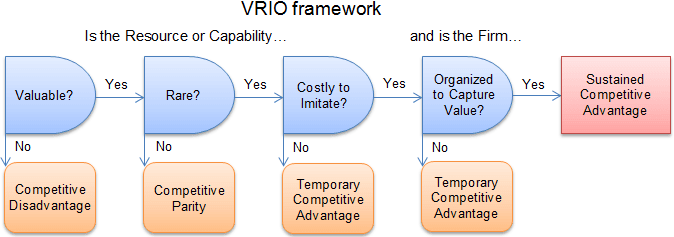
\includegraphics[width=0.8\textwidth]{vrio_framework}
 	\caption[The VRIO framework]{The VRIO framework. Adapted from~\citep{rothaermel2012strategic}}\label{fig:VRIO}
\end{figure}

The VRIN framework developed in~\cite{Barney:1991ur} was also extended and improved upon~\citep{Barney:1995tz} just as he had improved on the terminology of \rbt.
\cite{Barney:1995tz} introduced the concept of \acrshort{VRIO} to improve on \acrshort{VRIN}
\begin{description} 
   \setlength{\itemsep}{1pt}
\item[The Question of Value] Resources are valuable if they help organisations to increase the value offered to the customers. This is done by increasing differentiation or/and decreasing the costs of the production. The resources that cannot meet this condition, lead to competitive disadvantage.

\item[The Question of Rarity] Resources that can only be acquired by one or few companies are considered rare. When more than few companies have the same resource or capability, it results in competitive parity.

\item[The Question of Imitability] A company that has valuable and rare resource can achieve at least temporary competitive advantage. However, the resource must also be costly to imitate or to substitute for a rival, if a company wants to achieve sustained competitive advantage.

\item[The Question of Organisation] The resources itself do not confer any advantage for a company if it’s not organised to capture the value from them. Only the firm that is capable to exploit the valuable, rare and imitable resources can achieve sustained competitive advantage\footnote{adopted from~\citep{Strategic-management-insight:2013}}.
\end{description}

The key improvement to the VRIO (see also~\ref{fig:VRIO}) framework from the VRIN framework is the addition of the question if the organisation is ready and capable to exploit all the resources~\citep{Barney:1995tz,Strategic-management-insight:2013}.
The general thinking is this should lead to~\ca through \gls{FSA}~\citep{Barney:1991ur,Barney:2001tj,Barney:2011jp}. 
The frameworks by~\cite{Barney:1991ur,Barney:1995tz} lead to the following \wpro:

\begin{WP}\label{wp:rbt}
  The diversity in internal resources (humans and knowledge) within firms could be responsible for the heterogeneity of firms responses to changes institutional environment
\end{WP}

\subsection{Firm specific resources}

A key concept of~\citep{Barney:1991ur,Barney:2001tj} is that the different (internal) resources lead to~\glspl{FSA}.
The resources of MNE are by definition located in the host and home country of that MNE\@. 
\cite{Barney:1991ur,Barney:1995tz} suggests that ``resources within the firm are not perfectly mobile across firms and that heterogeneity can be long lasting''~\citep{Barney:1991ur}.
Whether this assumption holds true is a matter of discussion.
The fact that resources might be (perfectly) mobile given certain constraints has been brought up~\citep{Lavie:2006up,Priem:2001vd} already.\\
\cite{Hu:1995vg} identified that the firm's advantages are indeed transferable, be it with varying amounts of success (certain constraints).
The success can be made visible through the expansion of Hong Kong based firms in East Asia~\citep{Hu:1995vg}.
However the accomplishments of the same firms in their expanse into the US or Great Britain yielded a very different story~\citep{Hu:1995vg}.\\
The same holds for (high-tech) Korean firms expanding to \glsfull{EE} vis-a-vis expanding to  \glsfull{AE}. 
Different strategies were observed while sill dealing with comparable MNEs~\citep{Erramilli:1997wu}.
The same firm specific resources were employed in different capacities relative to the market that was entered.\\
Not only the economic regions that are entered are relevant to the methods and impact resources have on the MNE\@.
The type of resource has a profound effect on its capacity to be either internationally mobile or immobile~\citep{Tseng:2007wm}.\\
Some \glspl{FSA}, in the form of resources, have different characteristics in general. 
\cite{Rugman:2001ti} differentiates between three types of resources.
\begin{enumerate}[(a)]
   \setlength{\itemsep}{1pt}
\item Non location bound \fsa
\item Location bound \fsa 
\item Subsidiary specific advantages
\end{enumerate}
Where the (non) location bound \fsa are in it self to be exploited globally and easy to diffuse locally (a) or hard to exploit globally and provide local national responsiveness (b) the subsidiary specific advantages are a different matter by itself. 
They are easy to deploy globally but difficult to exploit internally~\citep{Rugman:2001ti}.
The subsidiary specific advantages display characteristics of perfectly mobile resources as they are very mobile across firms, but not within firms or MNEs.\\
The observations above relax the statement of~\cite{Barney:1991ur} somewhat as to the perfect mobility of resources.
According to~\citep{Rugman:2001ti,Tseng:2007wm,Erramilli:1997wu,Hu:1995vg,Rugman:1992uj} some consideration has to be given to the fact that resources are perfectly immobile according to \rbt.
This may not be always a certainty and depends off course, on a case by case basis as indicated above.
 
%The theory of Barney is \emph{introspective}. 
%It takes into account what is happening inside the firm.
%What knowledge is available, the people matter. 
%Processes that have been created over time are a contributing factor. 
%In the 1970's Toyota engineered \gls{tpm} for it's factories this gave them \gls{CA} over their US rivals as production cost were lower for their products.
%Only if these resources cannot be imitated in an other country and location this can create a \gls{CA}.
%In contrast to~\gls{RBV} the theory of~\cite{Porter:1980to} is thus~\emph{extrospective} and does not consider the company itself.\\
%Actually both theories are not mutually exclusive. They are very well capable of existing simultaneously. 
%This line of thought give rise to the fact that there might be a third pillar in strategy thinking.

%\section{Conclusions}

From an theoretical standpoint the \gls{WTO} can certainly be seen as an institution.
As a rules setting body the \wto~does certainly qualify as an institution and by setting these roles it tries to reduce the uncertainty for organisations.
The institutional characteristics are certainly very visible in the Formulation Phase of the \wto~life cycle. 
The outcome of the institution changes, their result, is most visible in the implementation phase.
This is the moment where the organisations (firms) have to respond to the new landscape. 
Their context has changed.
This is best theorised by the \gls{IBV}~and more to the point the strategy tripod~\cite{Peng:2009vt} and shown in figure~\ref{fig:Peng2009}.
The manner in which the firms respond to the changing context is not only dependant on the context, country and state and stage of the economy, but also has to do with the available resources and the industry of the firm is competing in. \\
The possible differences and similarities will be investigated in the next section.%

